\chapter{System Analysis}

\section{Problem Statement}

Industrial and construction sites are inherently high-risk environments where the failure to detect hazards promptly can lead to severe injuries or fatalities. Traditional monitoring methods, such as manual human supervision and retrospective CCTV review, are reactive by nature. They are limited by human attention span, visual coverage gaps, and the latency between an incident occurring and a response being initiated.

In addition to acute incidents such as falls or collisions, workers are also exposed to long-term \textbf{musculoskeletal risks} arising from repetitive, awkward, or sustained postures (e.g., excessive trunk flexion, overreaching, and asymmetric loading), which often remain undocumented and undetected by traditional monitoring practices.

\textbf{VisionSafe 360} is proposed as an automated, privacy-preserving solution designed to transform existing RTSP CCTV infrastructure into an active safety assistant. By leveraging Edge AI, the system detects four primary categories of safety hazards—\textbf{PPE violations}, \textbf{fall events}, \textbf{unsafe proximity}, and \textbf{posture-related ergonomic risks}—in near real-time. The primary objective is to shift industrial safety practices from \textbf{reactive investigation} to \textbf{proactive prevention}, utilizing localized interfaces tailored for the target operating environment.

\section{Problem Analysis}

\textbf{A. Constraints on Time and Resources}

\textbf{System Optimization:} Real-time operation mandates highly optimized inference pipelines. The target throughput is \textbf{15–30 FPS} for optimized models, though actual performance is contingent on model complexity, input resolution, and hardware acceleration.

\textbf{Hardware Sizing (Prototype Estimates):} Based on prototype testing, the approximate resource requirements are estimated at \textbf{\textasciitilde{}2 GB GPU VRAM and \textasciitilde{}2.4 GHz CPU per active camera stream}. These figures serve as capacity planning estimates; the system is designed to scale dynamically (e.g., via frame skipping or clustering) based on available compute power.

\textbf{Data Reliability:} Variability in industrial lighting, occlusion, and camera angles necessitates robust dataset curation and per-site threshold calibration to minimize false positives, both for acute hazard detection and for reliable estimation of \textbf{posture-related musculoskeletal risks} across diverse operating conditions.

\textbf{B. Safety and Operational Barriers}

\textbf{Surveillance Fatigue:} Human operators cannot maintain continuous, error-free attention across multiple video feeds for extended periods.

\textbf{Reactive Latency:} Post-incident video review is valuable for forensics but fails to prevent immediate harm.

\textbf{Documentation Burden:} Manual incident reporting is time-consuming and prone to human error. Automation is required to produce accurate, audit-ready logs covering both acute events (falls, PPE, proximity) and prolonged exposure to \textbf{ergonomically harmful postures}.

\textbf{C. Current Solutions and Limitations}

\textbf{Manual Supervision:} Effective only for small, contained areas; lacks scalability.

\textbf{Cloud-Based AI:} Often requires streaming raw video off-site, raising significant concerns regarding \textbf{bandwidth costs} and \textbf{data privacy}. Latency in cloud uploading can also delay critical alerts.

\textbf{D. Technological Challenges}

\textbf{Real-Time Processing:} The system must perform unified hazard detection—covering object detection, tracking, posture estimation, and rule evaluation (e.g., proximity logic)—concurrently within a sub-second latency budget.

\textbf{Privacy Compliance:} To comply with data protection standards, \textbf{on-edge anonymization (face blurring)} is mandatory before any visual data is persisted or transmitted. This also applies to posture analysis: only anonymized skeletal keypoints and ergonomic scores are propagated to the backend, not raw images.

\section{Project Feasibility Study}

\textbf{A. Technical Feasibility}

The system is built upon a proven open-source stack: \textbf{Python}, \textbf{OpenCV} (video ingestion), \textbf{Ultralytics YOLOv8} (object detection), and \textbf{FastAPI} (backend services). The architecture utilizes \textbf{Edge Computing} for critical inference, ensuring feasibility even in bandwidth-constrained environments.

In addition to PPE, fall, and proximity detection, the Edge AI stack is extended with a \textbf{Posture \& Ergonomic Analysis sub-module}. This module relies on skeletal keypoint extraction (e.g., from a lightweight pose estimation network) and rule-based ergonomic evaluation to approximate posture-related risk levels in real-time.

Within the Edge AI Engine, all four hazard categories—PPE violations, falls, unsafe proximity, and posture-related ergonomic risks—are evaluated in a unified pipeline. The engine not only detects the presence of hazards but also classifies their \textbf{severity} (e.g., high, medium, low), enabling a differentiated alert policy that reserves emergency alerts for acute hazards while treating posture hazards as low-severity, preventive signals. As with other AI components, all analysis runs locally on the Edge node, ensuring that raw video remains on-premises and only anonymized metadata is transmitted to the backend for long-term analysis.

\textbf{B. Economic Feasibility}

VisionSafe 360 leverages existing CCTV hardware, significantly reducing Capital Expenditure (CAPEX). The Return on Investment (ROI) is driven by the reduction in workplace accidents, lower insurance liabilities, and decreased administrative overhead for HSE teams, as well as by reducing long-term \textbf{musculoskeletal exposure} through preventive posture monitoring and ergonomic risk analysis.

\textbf{C. Legal Feasibility}

The design explicitly addresses privacy laws by performing local processing. No raw video streams are recorded or uploaded; only anonymized metadata and encrypted snapshots are retained, adhering to strict data privacy regulations for both acute incident data and long-term ergonomic posture records.

\textbf{D. Operational Feasibility}

The platform is designed to complement, not replace, existing HSE workflows. The localized Dashboard and Mobile App require minimal training, ensuring high adoptability by site supervisors and safety engineers, both for managing real-time incidents and for reviewing \textbf{posture-related ergonomic risk trends}.

\section{Project Time Scheduling}

The project follows a modular development lifecycle designed to allow parallel development of independent components (e.g., frontend and AI model training). The schedule is divided into six main phases:

\textbf{Requirements Analysis \& Dataset Preparation:} Defining scope and collecting diverse industrial datasets, including scenarios for PPE, falls, unsafe proximity, and representative working postures with ergonomic implications.

\textbf{Prototype Edge Inference Development:} Building the core detection engine.

\textbf{Backend Services \& Database Design:} Implementing the API gateway and storage schema.

\textbf{Real-time Alerting \& Mobile Integration:} Connecting the Edge engine to user devices.

\textbf{Dashboard Analytics \& Reporting:} Developing the visualization layer, including safety indicators and \textbf{ergonomic risk reports}.

\textbf{Integration Testing \& Validation:} Full system stress testing.

\begin{figure}[H]
\centering
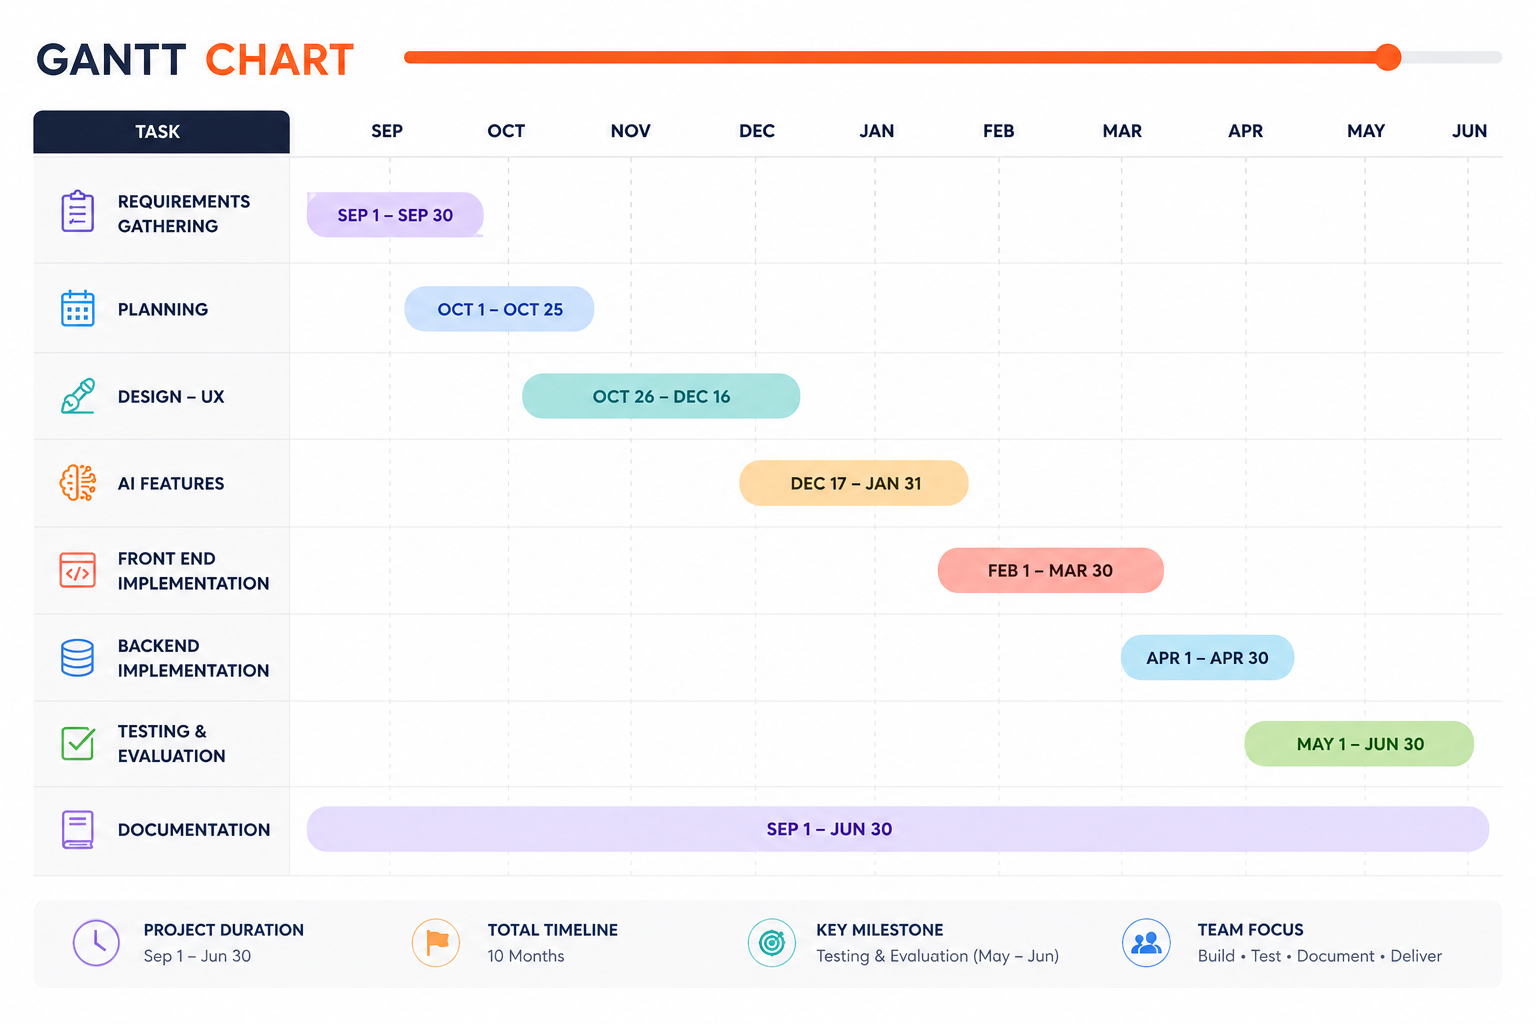
\includegraphics[width=0.95\linewidth,height=0.72\textheight,keepaspectratio]{images/img_033.png}
\caption{Gantt Chart of Project Schedule}
\end{figure}

\section{Functional Requirements}

\textbf{User Authentication \& RBAC:}

Secure login supporting distinct roles: \textbf{Admin}, \textbf{HSE Engineer}, \textbf{Site Supervisor}, and \textbf{Data Analyst}.

Admins possess full privileges for system configuration and user management.

\textbf{Camera Management:}

Admins can add/edit RTSP streams via the Dashboard.

System validates stream connectivity immediately upon entry.

Metadata includes: camera\_id, RTSP\_URL, ROI\_polygon, and location\_tag.

\textbf{Edge AI Engine (Internal Component):}

Autonomous execution of unified hazard inference pipelines for PPE detection, fall detection, unsafe proximity detection, and posture-related ergonomic risk analysis.

\textbf{Face Blurring:} Applied automatically to all detected persons prior to snapshot generation.

\textbf{Hazard Severity Classification:} For each detected hazard (PPE, fall, proximity, posture), the engine assigns an appropriate severity level (e.g., high, medium, low) based on confidence, duration, and hazard type. These severity levels are used by the alerting logic to differentiate between emergency incidents and low-severity ergonomic records.

\textbf{Real-Time Alerting:}

\textbf{Local (Emergency Incidents):} Immediate activation of on-site sirens/lights (latency <1s) \textbf{only} for acute, high-severity safety hazards, namely:

Confirmed fall events.

PPE violations (e.g., missing helmet or vest) above configured thresholds.

Unsafe proximity between workers and hazardous zones or moving equipment.

\textbf{Remote (Emergency Incidents):} Push notifications (FCM) to Supervisors and WebSocket updates to the HQ Dashboard are generated for the same set of acute, high-severity hazard types (falls, PPE violations, unsafe proximity).

\textbf{Non-Emergency Ergonomic Alerts:} Posture-related ergonomic hazards, typically classified as low or medium severity, are logged as \textbf{low-severity ergonomic events} and surfaced in dashboards and reports. They \textbf{do not} trigger sirens or high-priority mobile alerts, thereby avoiding alert fatigue while still providing actionable insights for preventive ergonomics.

\textbf{Event Management \& Lifecycle:}

Structured logging of incidents with timestamp, confidence score, computed severity, and snapshot.

\textbf{Closed-Loop Workflow:} Supervisors must "Acknowledge" alerts and record "Action Taken" to resolve an incident.

\textbf{Health Monitoring:}

Continuous tracking of camera status (Online/Offline), FPS, and connectivity.

Automated reconnection logic with exponential backoff.

\textbf{Privacy \& Retention:}

Strict policy: \textbf{No raw video storage}.

Configurable retention periods for snapshots and metadata, including both incident and ergonomic posture records.

\textbf{Posture \& Ergonomic Risk Assessment:}

The system shall continuously estimate worker body posture using skeletal keypoints extracted from video frames (e.g., shoulders, hips, knees, trunk orientation).

An internal ergonomic scoring mechanism (inspired by standard frameworks such as \textbf{RULA/REBA}) shall classify posture snapshots into low, medium, or high musculoskeletal risk levels.

Non-emergency \textbf{ergonomic alerts} shall be generated for prolonged high-risk postures (e.g., sustained trunk flexion beyond a configurable duration). These are logged as \textbf{low-severity events} and do not activate emergency sirens or high-priority mobile alerts.

Aggregated posture risk data (per worker zone or per camera) shall be stored as \textbf{ergonomic records} and made available to HSE Engineers for trend analysis and preventive intervention planning, helping identify high-risk tasks and areas over time without causing alert fatigue.

\section{Non-Functional Requirements}

\textbf{Performance:}

Target Inference Rate: \textbf{15–30 FPS} (hardware dependent).

End-to-End Latency (Detection to Mobile Alert): \textbf{2–3 seconds}.

\textbf{Scalability:} Horizontal scalability achieved by adding Edge nodes; vertical scalability via model optimization (e.g., quantization).

\textbf{Reliability:} The system must recover automatically from network interruptions and camera signal loss, for both real-time incident detection and continuous posture data collection.

\textbf{Security:}

Data in Transit: TLS/SSL encryption for API and WebSocket connections.

Data at Rest: Encrypted storage for snapshots; hashed passwords.

\section{System Actors and Roles}

\begin{table}[H]
\centering
\small
\renewcommand{\arraystretch}{1.2}
\begin{tabular}{|
>{\RaggedRight\arraybackslash}p{0.24\linewidth}|
>{\RaggedRight\arraybackslash}p{0.68\linewidth}|}
\hline
\textbf{Actor} & \textbf{Responsibilities} \\
\hline
System Administrator & System config, user management, camera setup, health monitoring. \\
\hline
HSE Engineer & Dashboard monitoring, incident investigation, compliance auditing, ergonomic trend analysis. \\
\hline
Site Supervisor & Receives mobile alerts, performs on-site intervention, logs corrective actions. \\
\hline
Data Analyst & Reviews long-term trends, generates safety KPIs and reports. \\
\hline
AI Engine & Internal System Actor. Performs unified hazard detection (PPE, falls, proximity, posture), anonymization, severity classification, and triggers events. \\
\hline
\end{tabular}
\caption{\textbf{System actors and roles}}
\end{table}

\section{Use Case Modeling}

\textbf{Use Case Diagram}

The Use Case diagram provides a high-level view of the system's functional scope and the interactions between actors and use cases. It clearly distinguishes between human actors (Admin, HSE, Supervisor) who interact with the UI, and the \textbf{AI Engine}, which is depicted as a system actor responsible for backend automation. A unified hazard detection use case covers all four hazard categories (PPE violations, falls, unsafe proximity, and posture-related ergonomic risks), while the alerting and reporting interfaces distinguish between emergency incident handling and preventive ergonomic analysis.

While the \textbf{AI Engine} executes hazard detection and posture analysis in a unified pipeline on the Edge node, only acute, high-severity hazards (falls, PPE violations, unsafe proximity) enter the emergency alerting workflow; posture-related deviations, typically of lower severity, are captured as ergonomic records and exposed through analytic views rather than immediate alarms.

\begin{figure}[H]
\centering
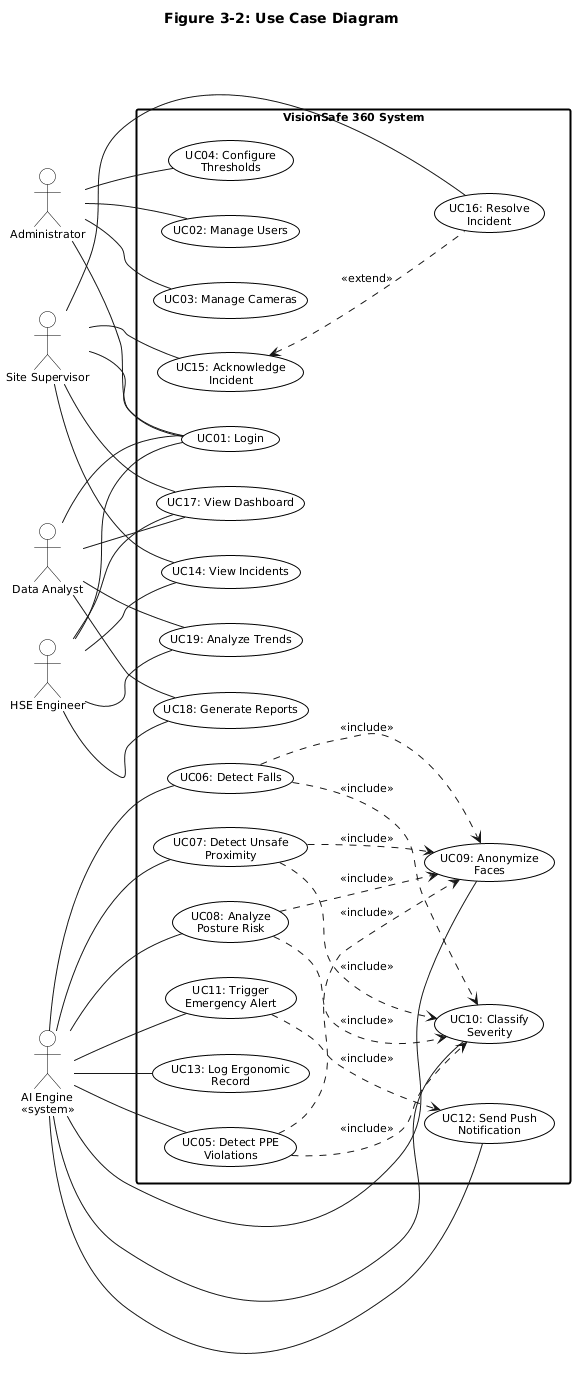
\includegraphics[width=0.95\linewidth,height=0.72\textheight,keepaspectratio]{images/img_007.png}
\caption{Key Use Case Scenarios}
\end{figure}

\textbf{Hazard Detection:} The Edge AI detects a "Fall". The system validates confidence, classifies severity, checks the cooldown timer, triggers the local siren, blurs faces in the frame, and uploads the event to the Backend as an emergency incident.

\textbf{Incident Resolution:} A Supervisor receives a notification, opens the app to view the snapshot, attends to the worker, and marks the incident as "Resolved" with notes.

\textbf{Camera Onboarding:} The Admin inputs an RTSP URL. The system attempts a connection handshake; if successful, the camera is added to the active monitoring pool.

\textbf{Posture Trend Analysis:} The AI Engine periodically evaluates worker posture using skeletal keypoints and assigns ergonomic risk scores (e.g., low/medium/high). These low-severity posture records are aggregated by camera or work zone and later reviewed by HSE Engineers through the dashboard to identify tasks or areas associated with sustained high ergonomic risk.

\section{Activity Diagram}

This diagram details the sequential logic flow of the core detection loop, specifically focusing on how the system handles continuous video frames. It illustrates the critical decision-making process: acquiring a frame, running unified hazard inference (PPE, falls, proximity, posture), validating the detections against confidence thresholds, and then classifying the \textbf{severity} of each hazard. This mechanism is vital to prevent "alert fatigue" by ensuring that only genuinely high-severity, acute hazards (e.g., a confirmed fall with high confidence) can trigger immediate emergency alerts.

In parallel, or rather as part of the unified hazard analysis, posture-related ergonomic hazards are evaluated and assigned typically low or medium severity levels. These posture hazards generate \textbf{non-emergency, low-severity posture records} for long-term musculoskeletal risk assessment. These posture-related records do not trigger real-time sirens or high-priority alerts but instead feed ergonomic dashboards and reports for HSE teams.

\begin{figure}[H]
\centering
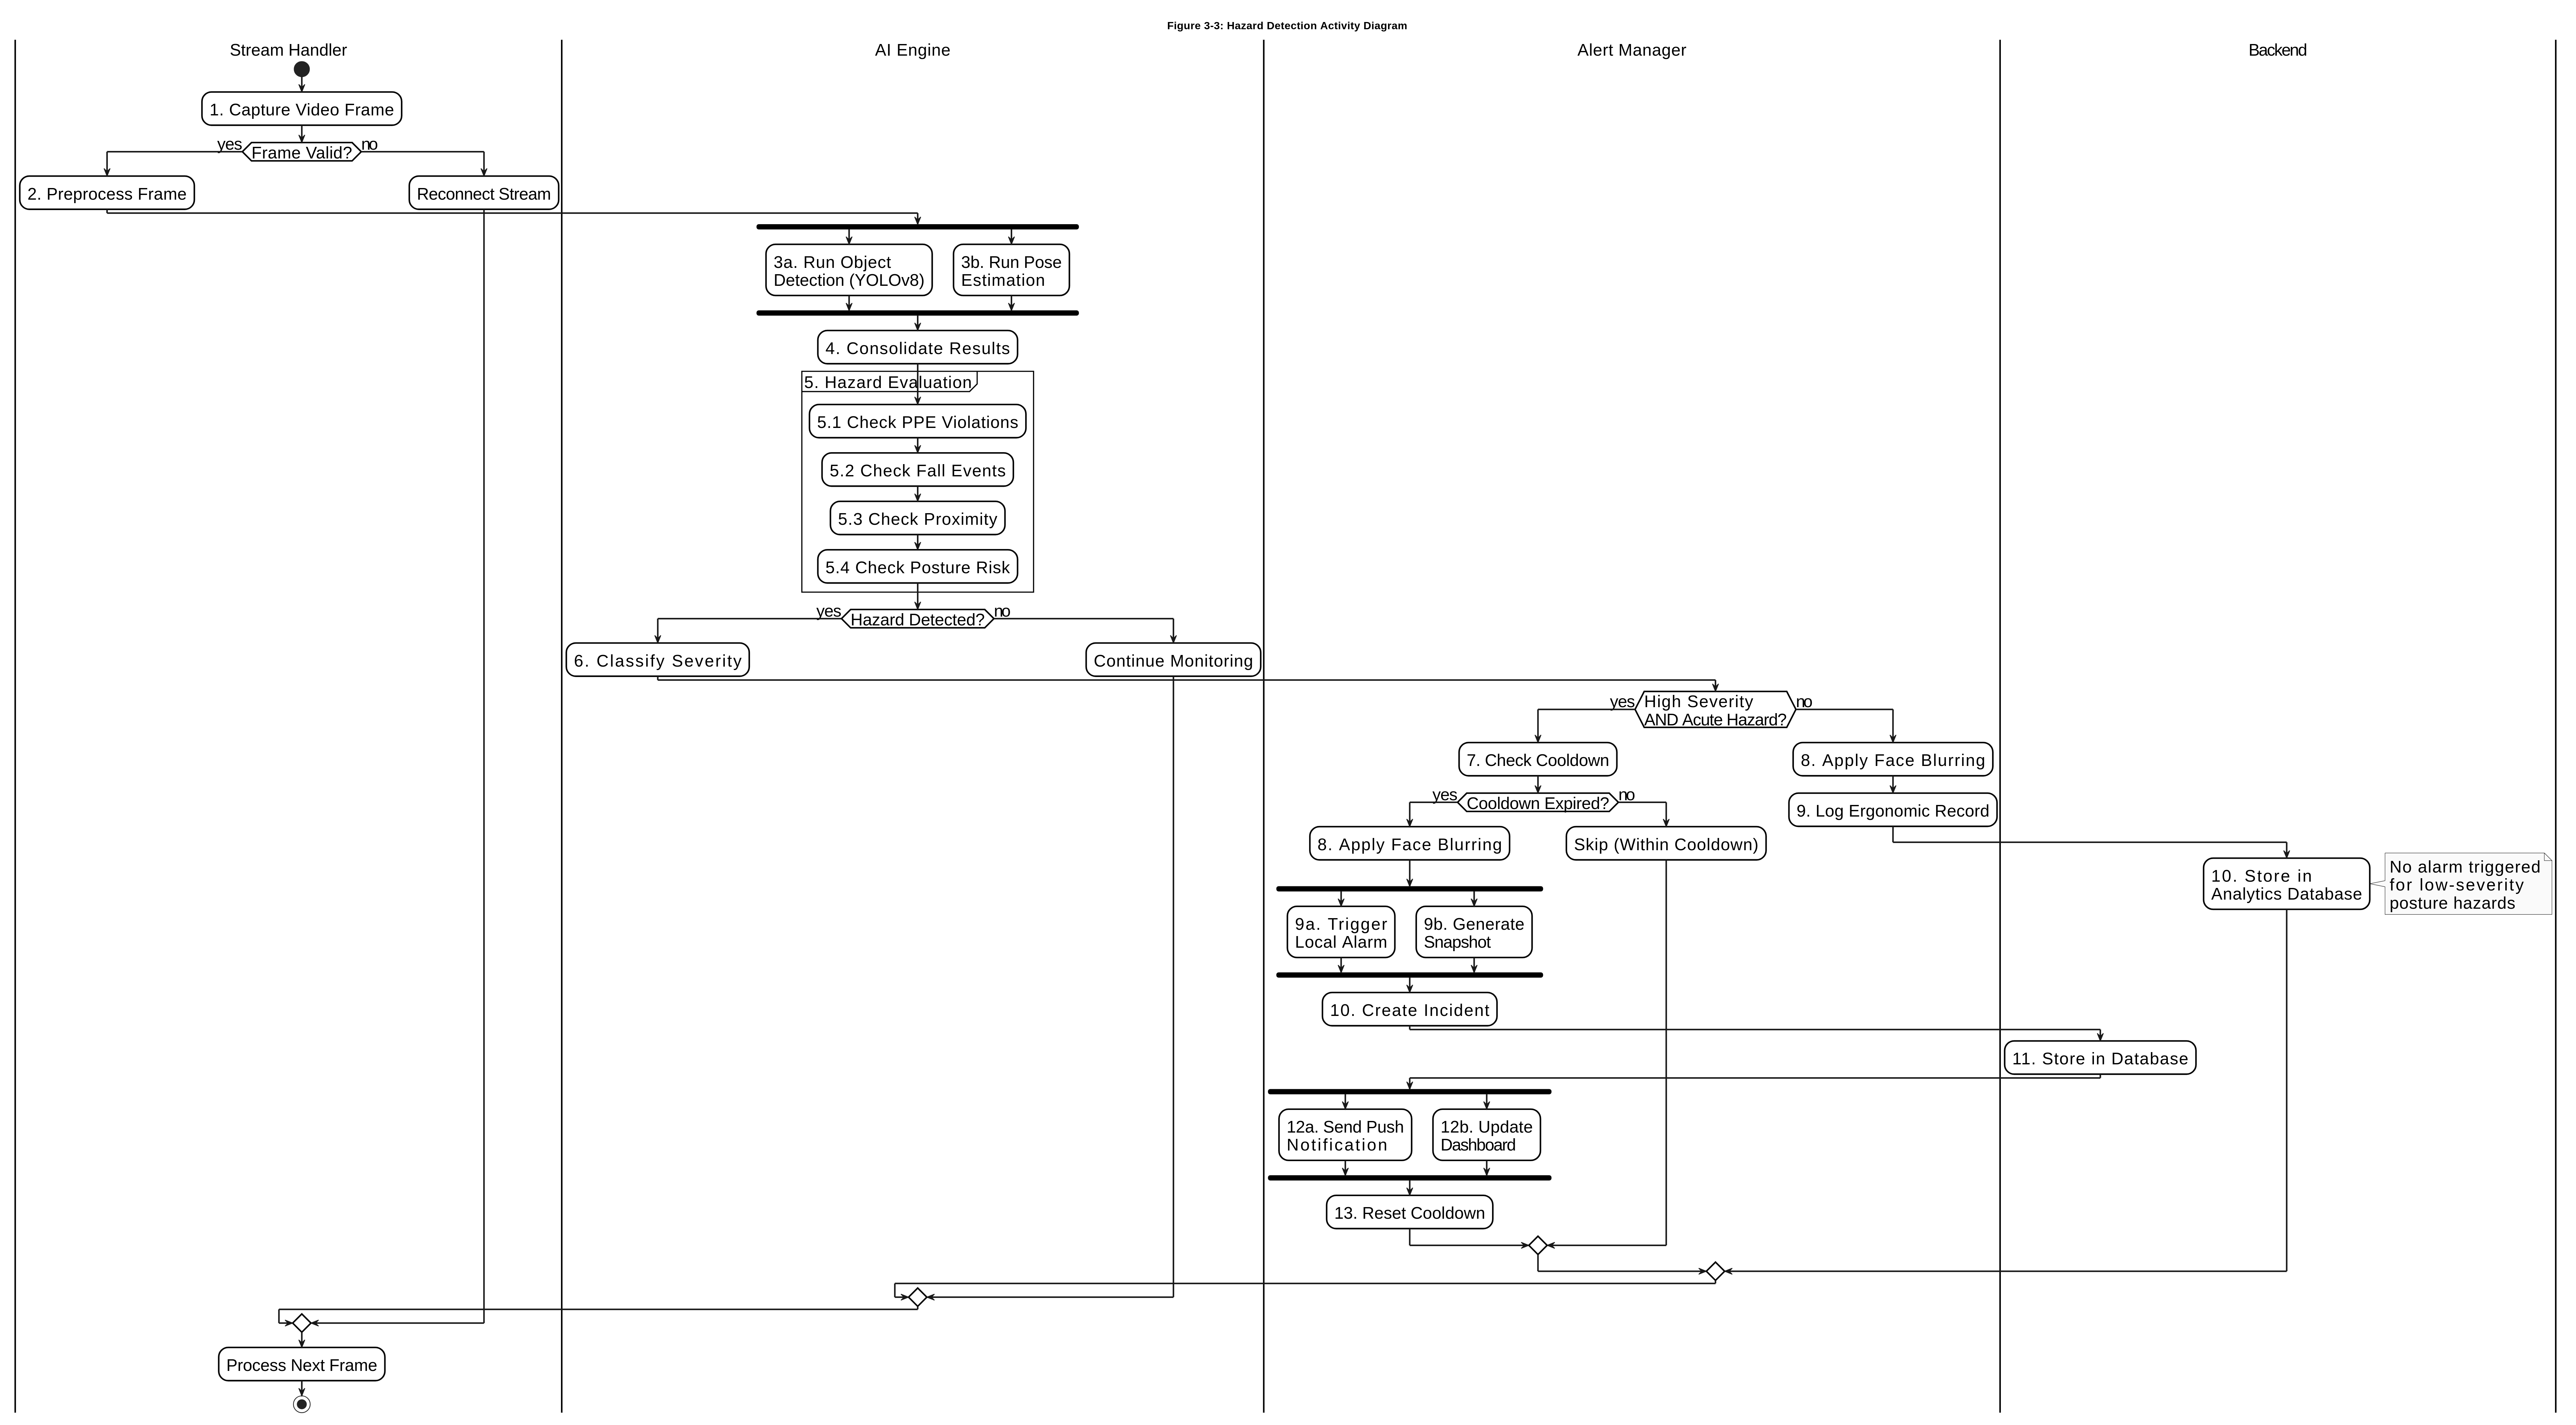
\includegraphics[width=0.95\linewidth,height=0.72\textheight,keepaspectratio]{images/img_008.png}
\caption{Activity Diagram}
\end{figure}

\textbf{Flow Summary:}

Capture Frame → Unified Inference (PPE/Fall/Proximity/Posture) → Hazard Evaluation → Severity Classification →

\textbf{If High/Critical \& Acute Hazard (PPE/Fall/Proximity):}

Cooldown Check → Trigger Alarm → Anonymize \& Save → Notify Backend (Incidents)

\textbf{Else (Low/Medium Severity, including most Posture cases):}

Log Ergonomic / Low-Severity Record → Notify Backend (Analytics/Ergonomics).

\section{Data Flow Diagram (DFD)}

\textbf{Level 0 (Context Diagram)}

The Context Diagram (Level 0) defines the system boundary of VisionSafe 360. It illustrates the external entities that interact with the system: \textbf{Cameras} (Input source), \textbf{Site Supervisors/HSE} (Notification recipients and ergonomic data consumers), and \textbf{Admins} (Configuration). The central process represents the entire VisionSafe system, abstracting internal complexities to focus on input/output data streams, including both real-time emergency incident alerts and longer-term ergonomic posture records.

\begin{figure}[H]
\centering
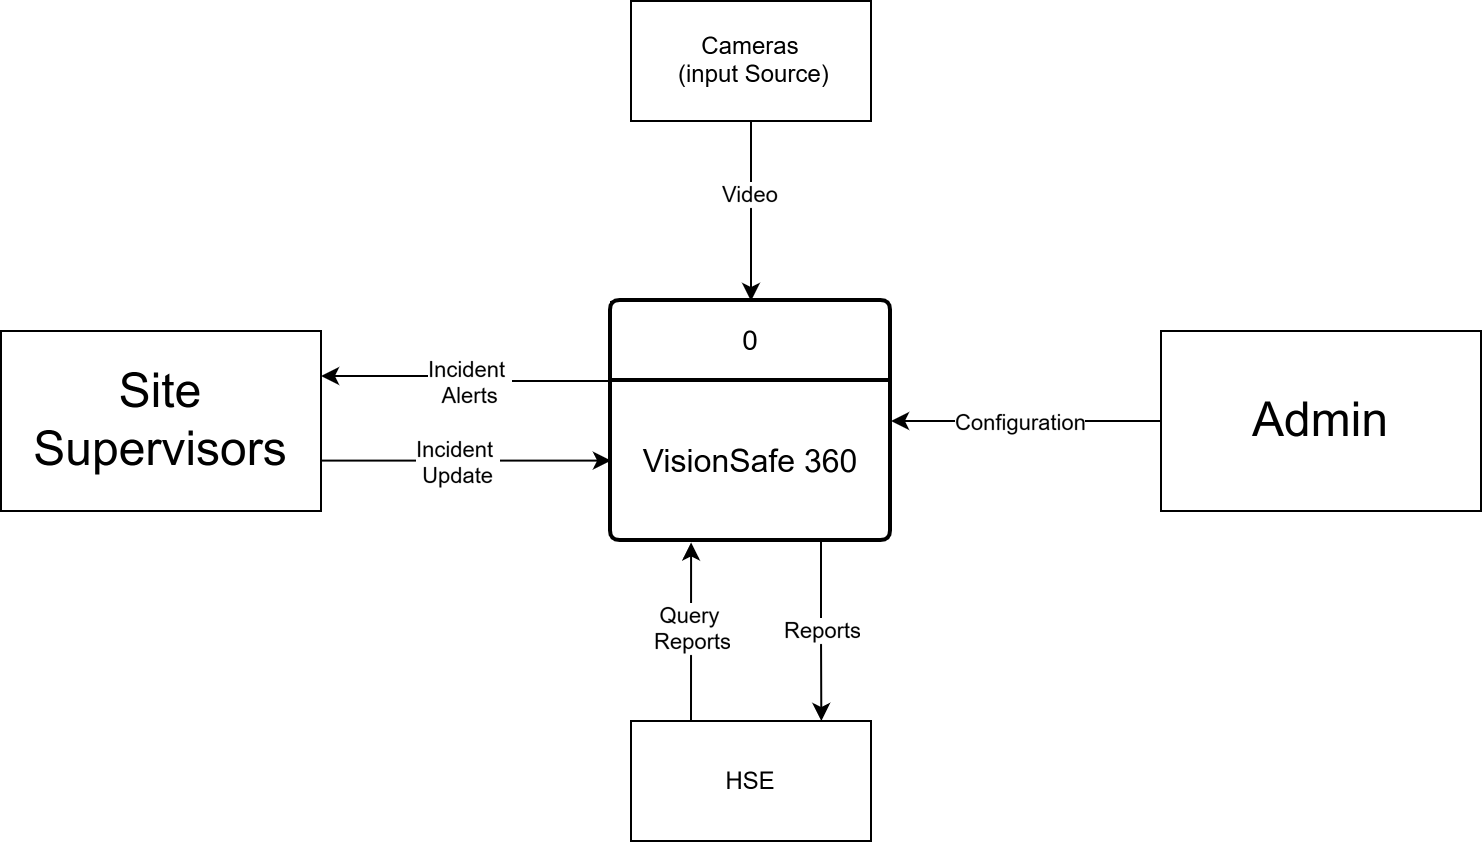
\includegraphics[width=0.95\linewidth,height=0.72\textheight,keepaspectratio]{images/img_009.png}
\caption{Context Diagram}
\end{figure}

\textbf{Level 1 Diagram}

The Level 1 DFD decomposes the system into its primary subsystems to show detailed data routing:

\textbf{Ingestion \& Processing:} RTSP streams enter the Edge module where unified hazard inference (PPE, falls, proximity, posture) and face blurring occur. Hazard evaluation and severity classification are applied to all hazard categories.

\textbf{Transmission:} Only metadata and encrypted snapshots are passed to the \textbf{API Gateway}. This includes both hazard metadata for acute, high-severity incidents (e.g., falls, PPE violations, unsafe proximity) and posture-related ergonomic scores and durations (typically logged as low-severity records for trend analysis).

\textbf{Storage:} Structured data is persisted in the SQL Database, with separate fields or records representing emergency incidents (e.g., falls, PPE violations) and non-emergency ergonomic observations (e.g., high-risk posture episodes).

\textbf{Presentation:} The Backend serves data to the Web Dashboard and pushes notifications to Mobile Clients. HSE Engineers can review both real-time emergency alerts (for acute hazards) and aggregated low-severity ergonomic posture trends to inform preventive interventions without overwhelming supervisors with immediate alarms.

\begin{figure}[H]
\centering
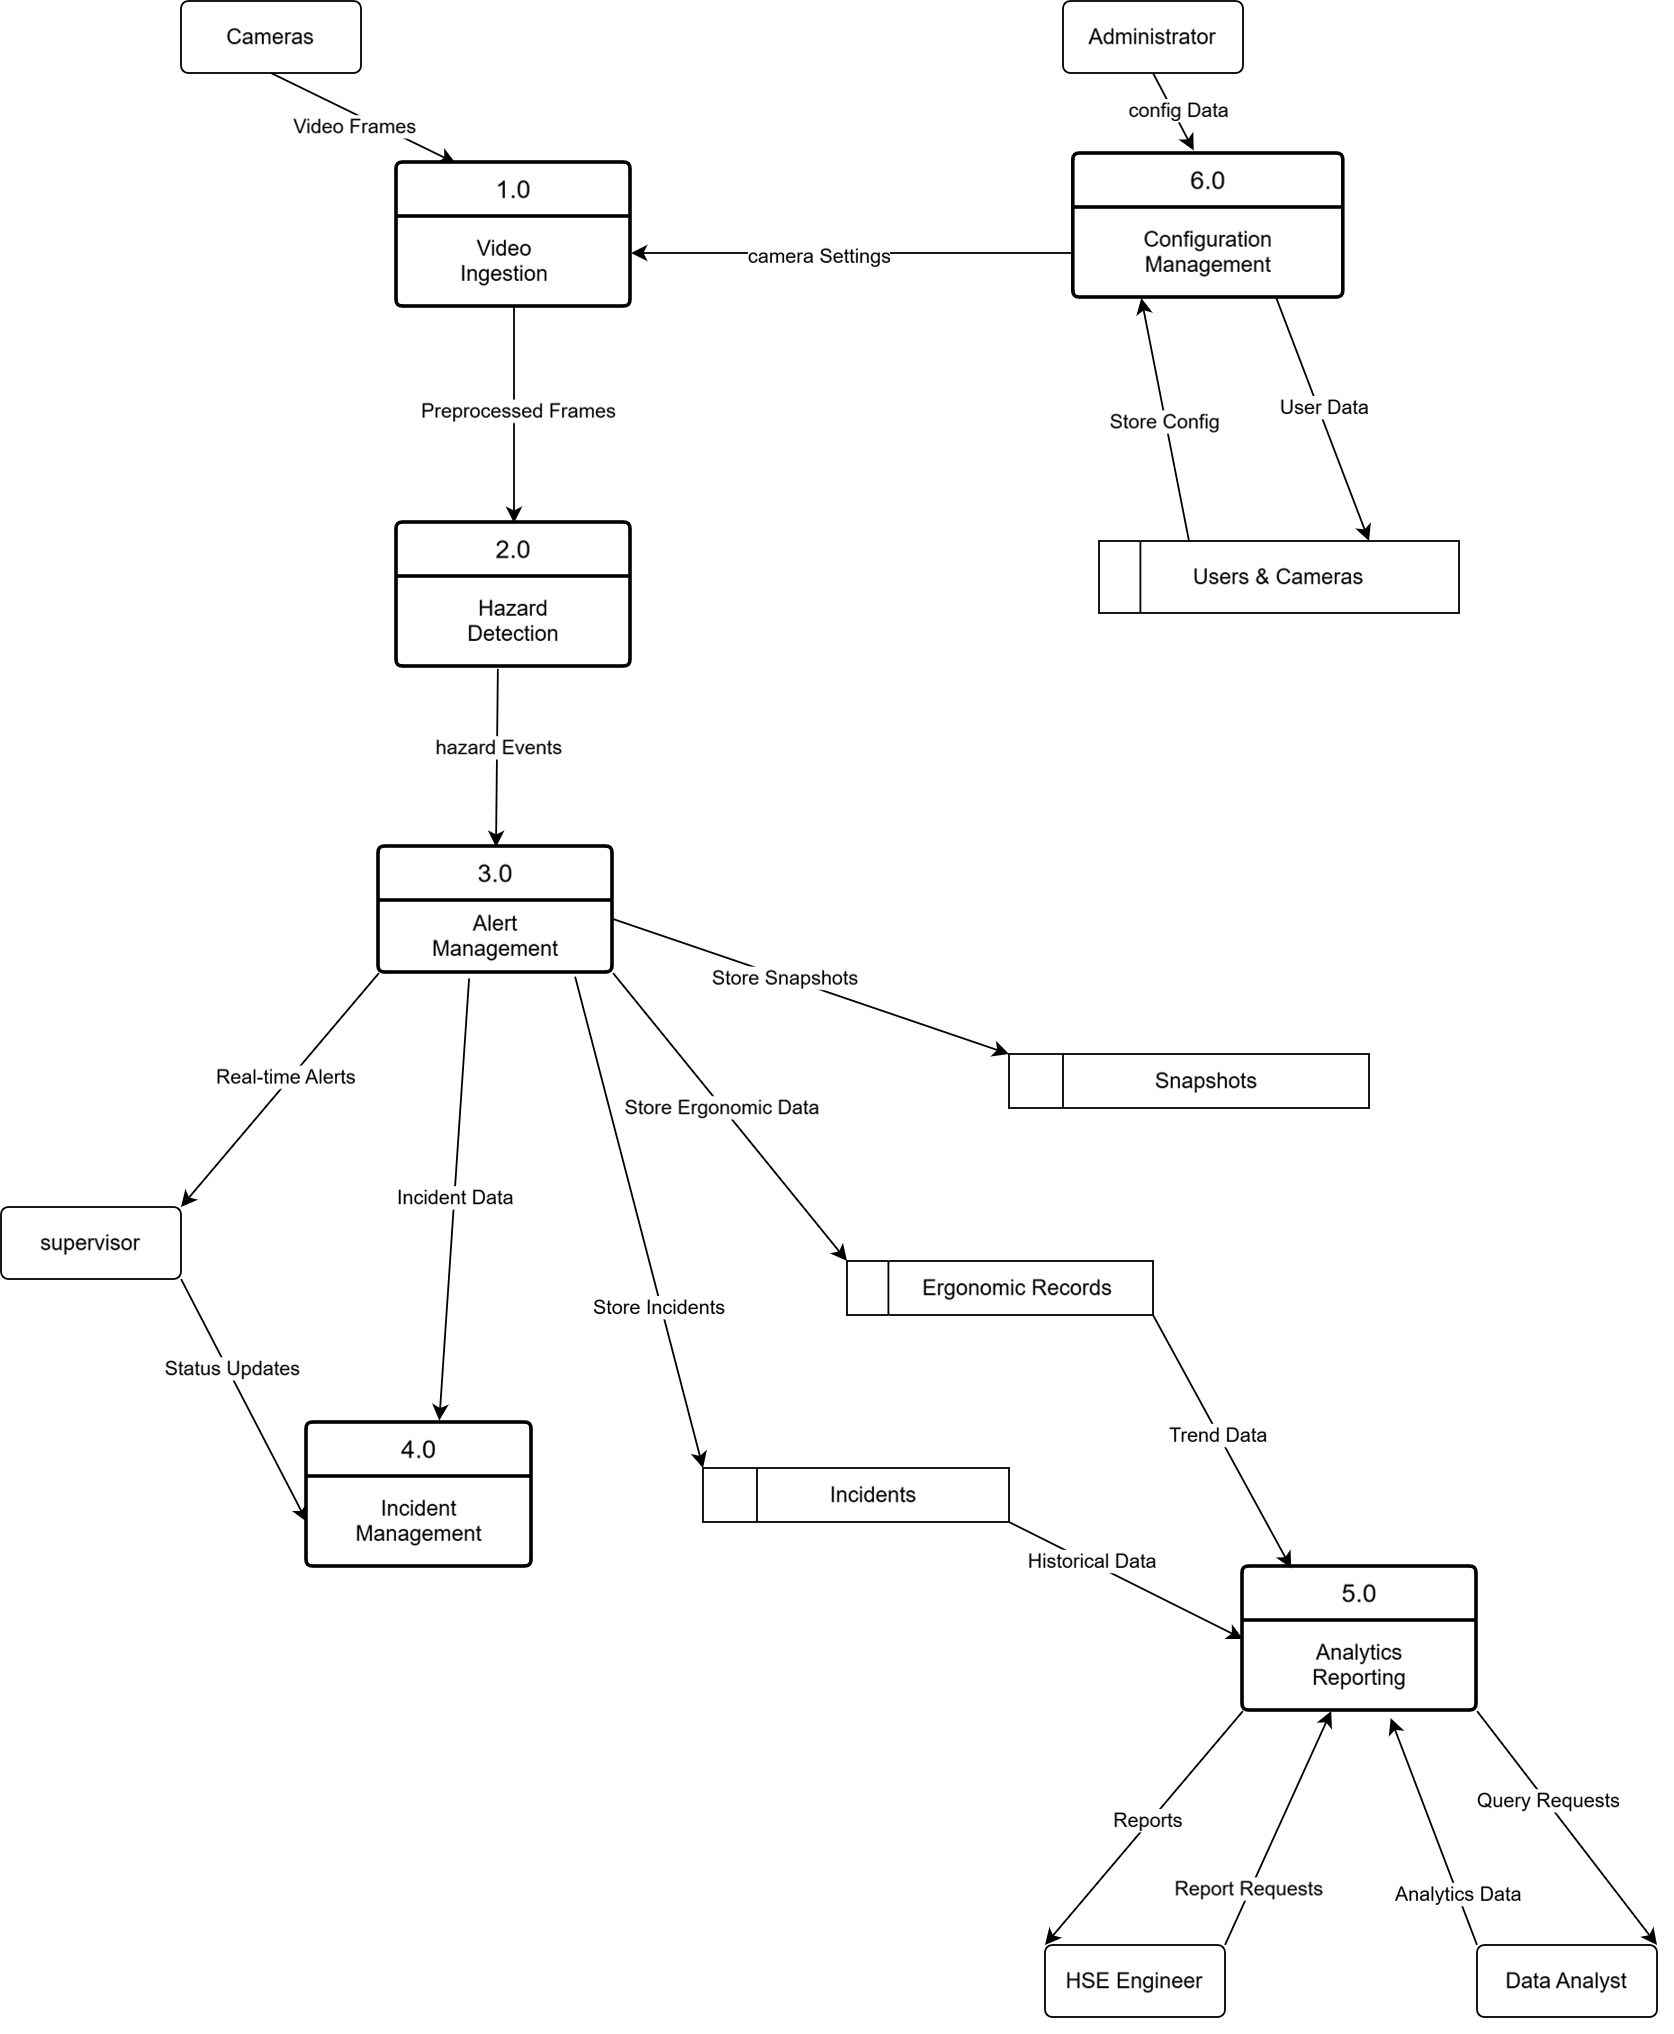
\includegraphics[width=0.95\linewidth,height=0.72\textheight,keepaspectratio]{images/img_010.png}
\caption{Data Flow Diagram (Level 1)}
\end{figure}

\section{Entity Relationship Diagram (ERD)}

The ERD visualizes the database schema designed to support the system's data persistence requirements. It employs a normalized relational structure to ensure data integrity. The central entity is the \textbf{Incident}, which links \textbf{Cameras} (where it happened), \textbf{Hazard Types} (what happened), and \textbf{Users} (who resolved it). This structure supports complex queries for analytics, such as "Total PPE violations per camera per week". Posture-related ergonomic risks are represented as hazard types of lower severity (e.g., POSTURE\_RISK) and can be queried independently or alongside other hazards to understand both acute and chronic risk patterns.

\begin{figure}[H]
\centering
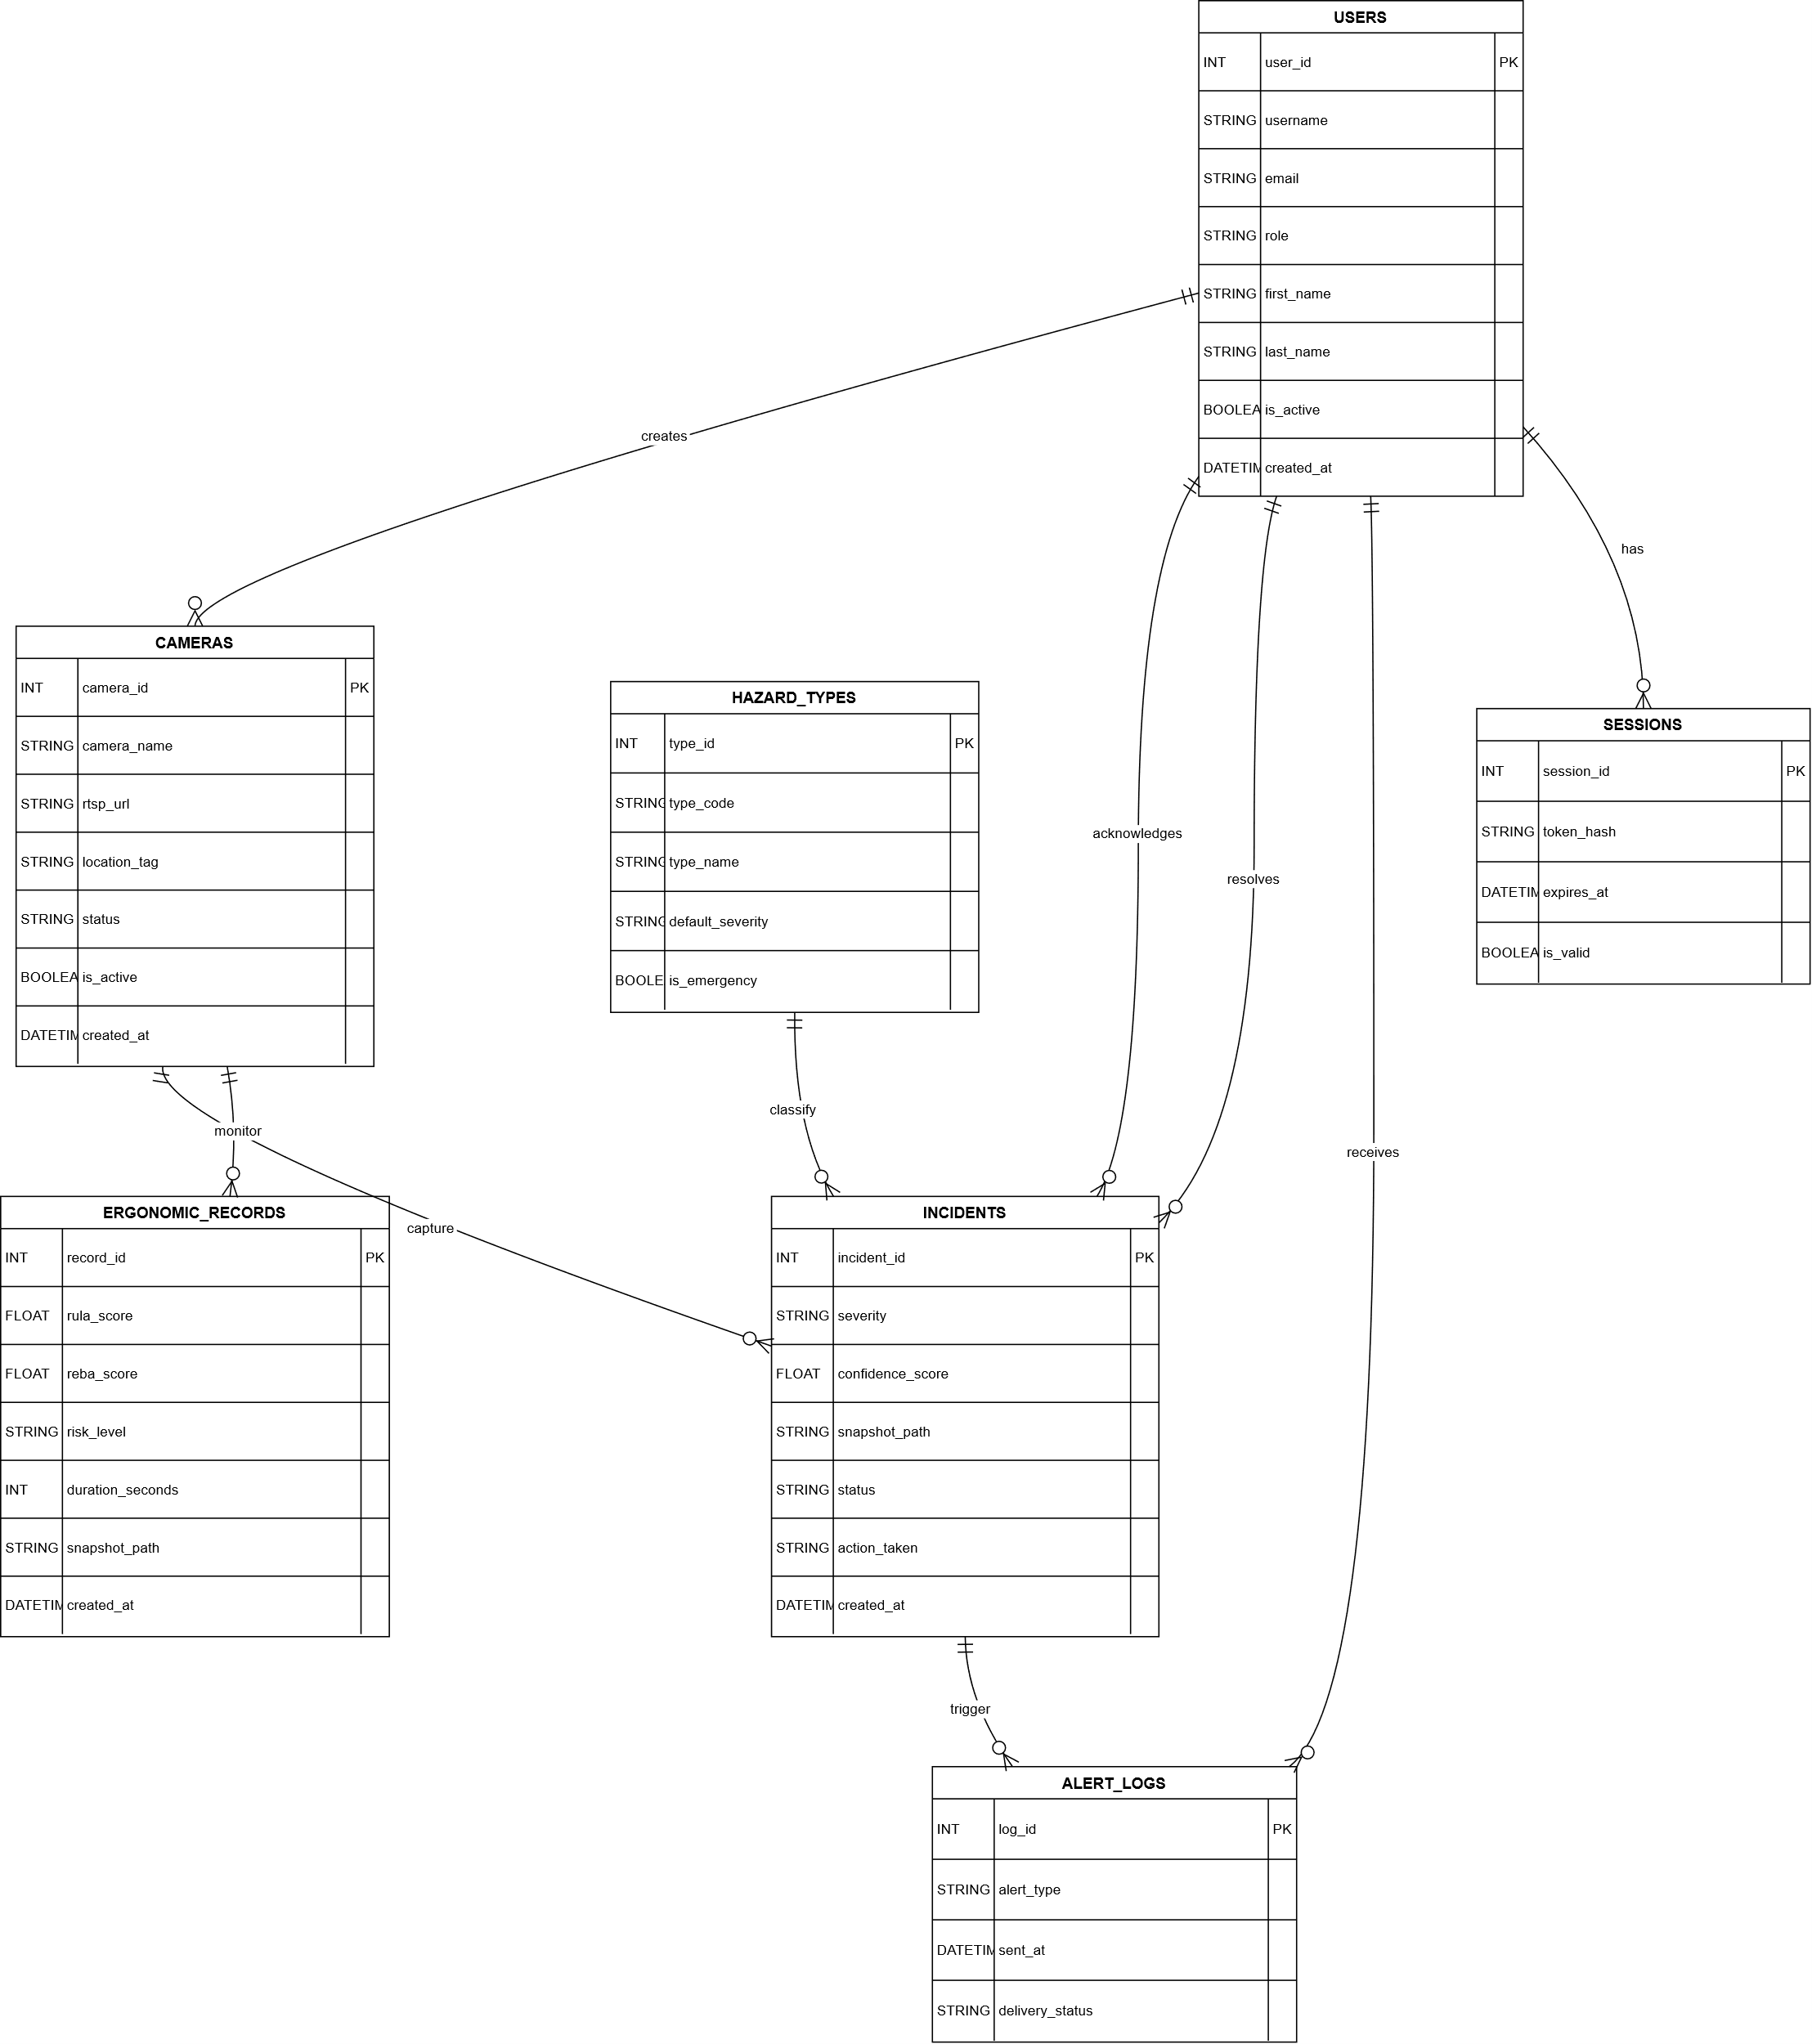
\includegraphics[width=0.95\linewidth,height=0.72\textheight,keepaspectratio]{images/img_011.png}
\caption{Entity Relationship Diagram}
\end{figure}

\textbf{Key Entities:}

\textbf{Users:} Stores authentication credentials, roles, and FCM tokens for mobile pushes.

\textbf{Cameras:} Contains configuration data including RTSP URLs and JSON-defined Region of Interest (ROI) polygons.

\textbf{Incidents:} The core transactional table storing event timestamps, confidence scores, severity, snapshot paths, and resolution status. This includes safety-critical events (e.g., falls) and may also reference posture-related events classified as low-severity when needed for ergonomic analysis.

\textbf{HazardTypes:} A lookup table defining detectable classes (e.g., "No Helmet", "Fall", "Proximity", "Posture Risk") and their associated default severitylevels.

\section{Class Diagram}

The Class Diagram represents the static structure of the software implementation, adhering to Object-Oriented Design (OOD) principles. It highlights the modular separation of concerns:

\textbf{StreamHandler:} Responsible solely for video I/O, frame buffering, and connection health.

\textbf{InferenceEngine:} Wraps the YOLO model (and any auxiliary pose estimation models), handling pre-processing and post-processing of tensors.

\textbf{HazardAnalyzer:} Contains the business logic for unified hazard evaluation (PPE, falls, proximity, posture). It generates hazard events enriched with type and severity information.

\textbf{PostureAnalyzer:} A dedicated analytic component that consumes frames and/or pose data to extract skeletal keypoints, compute ergonomic scores (e.g., RULA/REBA-inspired), and provide posture-related hazard candidates and risk levels to the HazardAnalyzer.

\textbf{Alerting/Notification Logic (e.g., AlertManager + NotificationService):} Applies an alert routing policy based on hazard severity and type:

High/Critical severity for acute hazards (falls, PPE, proximity) → emergency sirens and incident creation.

Low/Medium severity, especially posture-related ergonomic hazards → ergonomic records and analytic logging only (no sirens).

\textbf{NotificationService:} An interface for triggering external actions (Sirens, API calls) without coupling the core logic to specific output hardware.

The PostureAnalyzer and HazardAnalyzer jointly implement a unified hazard detection pipeline, while the alerting logic enforces different behaviors for emergency incidents versus low-severity ergonomic records.

\begin{figure}[H]
\centering
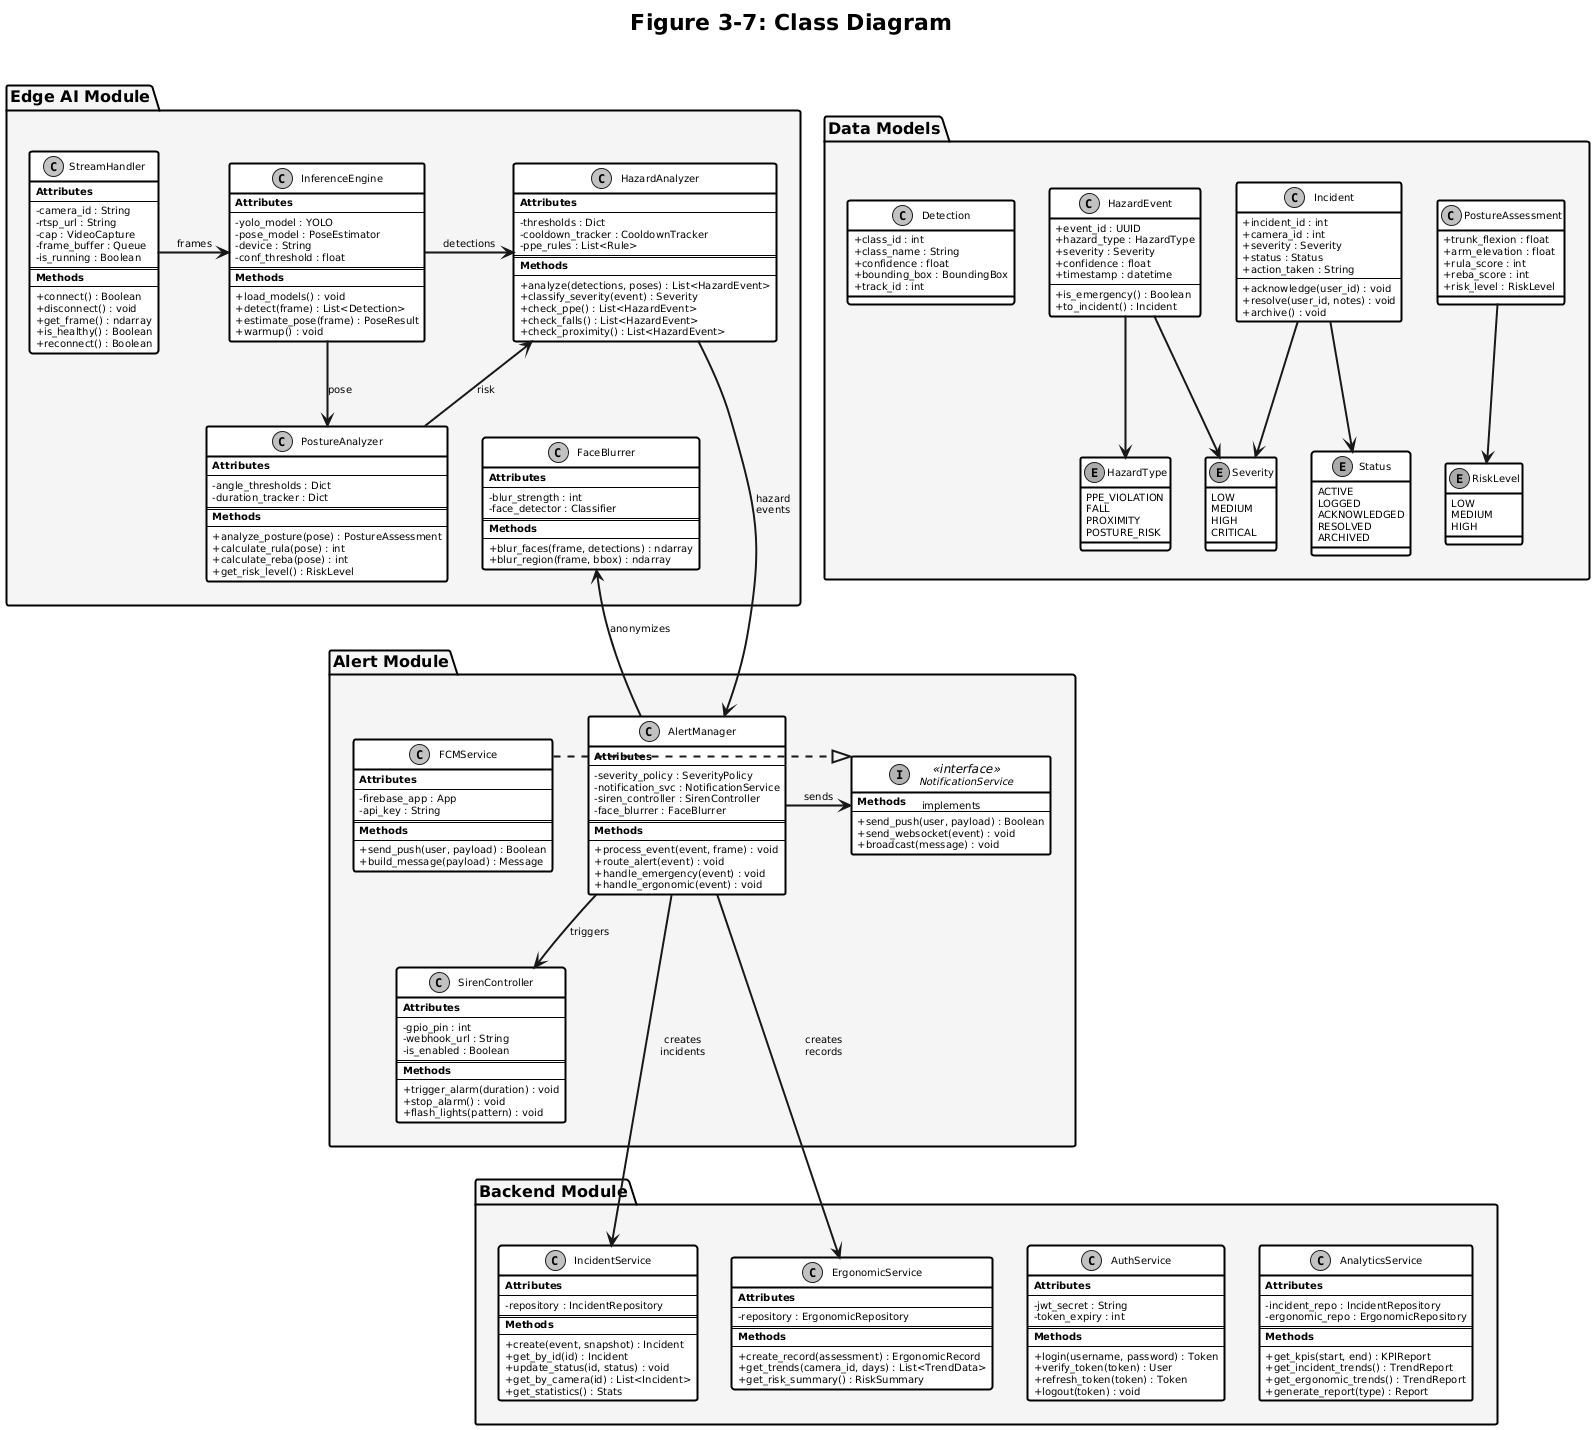
\includegraphics[width=0.95\linewidth,height=0.72\textheight,keepaspectratio]{images/img_012.png}
\caption{Class Diagram}
\end{figure}

\section{Sequence Diagram}

The Sequence Diagram provides a dynamic view of the system, capturing the chronological order of interactions during a "Hazard Detection" scenario. It traces the lifecycle of a single video frame: from capture by the \textbf{StreamHandler}, through unified hazard analysis by the \textbf{InferenceEngine}, \textbf{PostureAnalyzer}, and \textbf{HazardAnalyzer}, to the final alerts triggered (or not triggered) by the alerting logic and received by the \textbf{Mobile Client}.

In this workflow, a unified hazard event is created, containing both the hazard type (PPE, fall, proximity, posture) and its severity (e.g., high/medium/low). The alerting logic then decides whether this event becomes an emergency incident (with sirens and mobile alerts) or a low-severity ergonomic record suitable for trend analysis. This diagram is critical for understanding the latency and dependencies between the Edge and Backend components, as well as the separation between emergency incident handling (high-severity PPE/fall/proximity) and continuous, preventive ergonomic analysis (typically low-severity posture hazards) that avoids contributing to alert fatigue.

\begin{figure}[H]
\centering
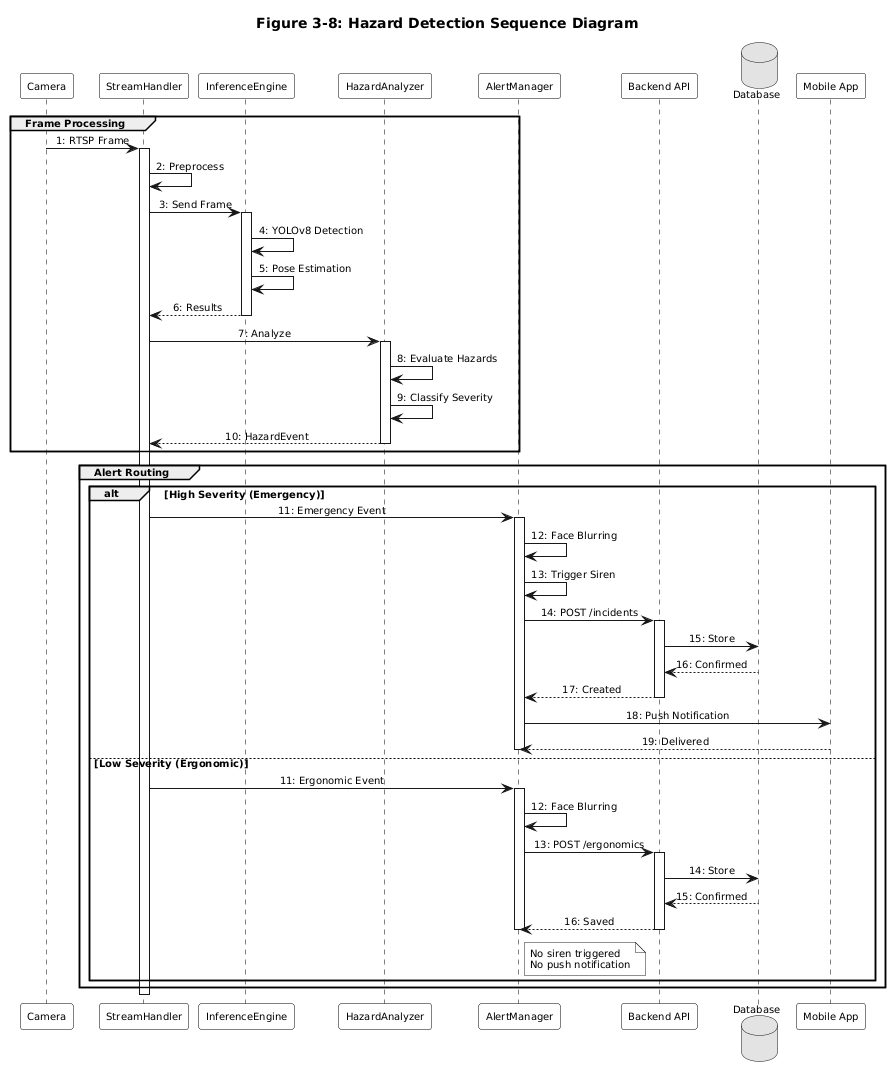
\includegraphics[width=0.95\linewidth,height=0.72\textheight,keepaspectratio]{images/img_013.png}
\caption{Sequence Diagram}
\end{figure}

\textbf{Sequence Steps:}

\textbf{StreamHandler} provides a frame to \textbf{InferenceEngine}.

\textbf{InferenceEngine} returns detection bounding boxes and pose-related keypoints to \textbf{HazardAnalyzer} and \textbf{PostureAnalyzer}.

\textbf{PostureAnalyzer} evaluates skeletal keypoints, computes ergonomic scores, and provides posture-related hazard candidates to \textbf{HazardAnalyzer}.

\textbf{HazardAnalyzer} consolidates PPE, fall, proximity, and posture-related inputs, confirms validity (rules + thresholds), and produces hazard events enriched with \textbf{hazard type and severity}.

The alerting logic (e.g., AlertManager + NotificationService) inspects each hazard event:

For high-severity acute hazards (e.g., falls, PPE, proximity), it triggers local hardware (sirens/lights) and posts an incident to the \textbf{Backend API}.

For low-severity posture-related ergonomic hazards, it bypasses sirens and posts an ergonomic record to the \textbf{Backend API} asynchronously.

\textbf{Backend} persists both emergency incidents and ergonomic records and pushes a real-time update to the \textbf{Mobile Client} (for incidents) and posture dashboards (for HSE Engineers).

\section{Incident Lifecycle \& State Transition}

This State Transition Diagram models the lifecycle of an Incident object, ensuring accountability and workflow enforcement. It defines how an incident moves from being a raw detection to a closed case. This prevents incidents from being "lost" and mandates human intervention for closure.

\begin{figure}[H]
\centering
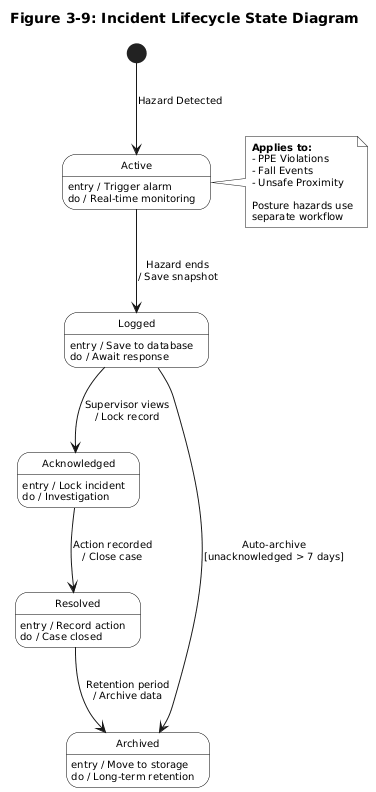
\includegraphics[width=0.95\linewidth,height=0.72\textheight,keepaspectratio]{images/img_014.png}
\caption{State Diagram}
\end{figure}

\textbf{Active:} The hazard is currently detected; alerts are firing.

\textbf{Logged:} The hazard has ceased or stabilized; the event is saved in the DB but requires attention.

\textbf{Acknowledged:} A Supervisor has viewed the notification (locking the incident).

\textbf{Resolved:} Corrective action has been logged, and the case is closed.

\textbf{Archived:} Old data is moved to cold storage for long-term retention.

The Incident lifecycle focuses on acute, high-severity, safety-critical events (such as PPE violations, falls, and unsafe proximity). Posture-related ergonomic observations, typically classified as low or medium severity, are treated as \textbf{non-critical records} and do not enter the emergency incident lifecycle. Instead, they are stored as ergonomic events associated with cameras or work zones, supporting long-term analysis and preventive ergonomics rather than immediate alarm escalation.

\section{Component Diagram}

The Component Diagram illustrates the high-level modular decomposition of VisionSafe 360 and clarifies the responsibilities and interfaces between subsystems across the Edge and Backend environments. It emphasizes the system’s design principle of keeping safety-critical inference and privacy enforcement on-premise (Edge), while delegating persistence, analytics, and multi-client distribution to the Backend.

At the Edge Node, the Stream Handler ingests RTSP camera streams and provides frames to the AI Engine for unified hazard inference. The Posture Analyzer operates alongside the core inference pipeline to estimate skeletal keypoints and compute ergonomic risk indicators, which are then consolidated within the hazard evaluation flow. Prior to any persistence or transmission, the Face Blurring component enforces privacy by anonymizing detected persons. An Alert Controller orchestrates event routing, ensuring that high-severity acute hazards trigger local alarms (via GPIO) while posture-related ergonomic risks are typically logged as low-severity records for trend analysis.

On the Backend Server, an API Gateway exposes secured endpoints and routes requests to specialized services, including Authentication, Incident Management, Ergonomic Records, and Analytics. Data persistence is handled through a dedicated Data Layer, where structured records are stored in PostgreSQL, frequently accessed data is optimized using Redis cache, and encrypted snapshots are stored in file storage. External services such as Firebase FCM are integrated to deliver push notifications to client applications, including the Mobile App and Web Dashboard.

\begin{figure}[H]
\centering
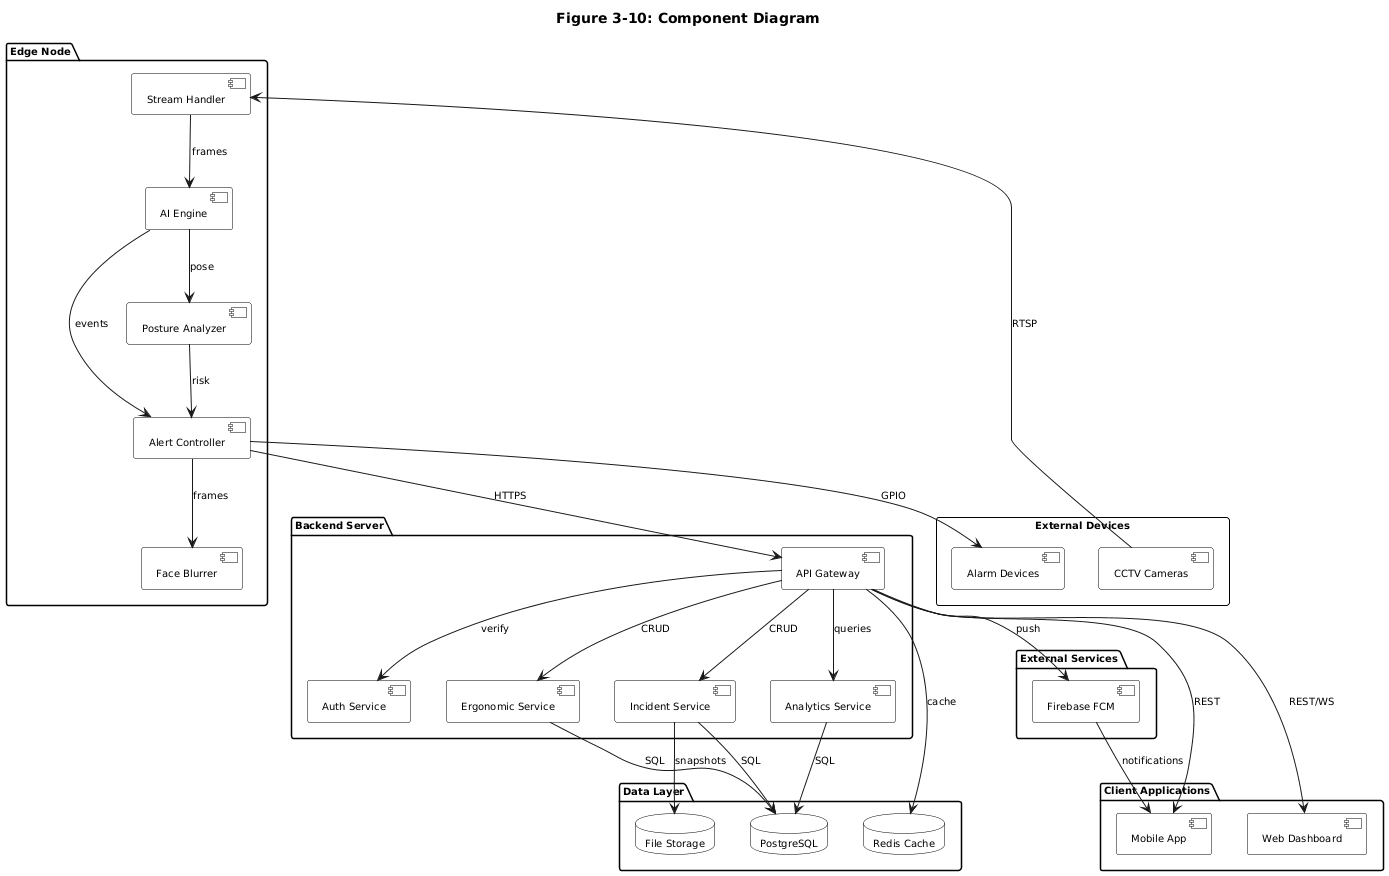
\includegraphics[width=0.95\linewidth,height=0.72\textheight,keepaspectratio]{images/img_015.png}
\caption{Component Diagram}
\end{figure}

\section{Deployment Diagram}

The Deployment Diagram presents the physical runtime topology of VisionSafe 360 across an industrial site and cloud infrastructure. It highlights how the system integrates with existing CCTV installations while ensuring low latency for emergency response and preserving privacy by keeping raw video on-site.

Within the Industrial Site, multiple IP cameras stream video over RTSP to the Edge Server (e.g., NVIDIA Jetson). The Edge node hosts the core runtime modules—stream handling, inference execution, and alert management—along with the primary AI models (YOLOv8 for detection and a lightweight pose model for posture estimation). For immediate on-site response, the Edge Server interfaces with the Alarm System (e.g., siren and strobe light) through GPIO, enabling sub-second activation for confirmed high-severity hazards.

The Cloud Infrastructure hosts the application layer responsible for orchestration and user-facing services, including the FastAPI Backend and a WebSocket server for real-time dashboard updates. Persistent storage is provided through PostgreSQL for structured incident/ergonomic records, Redis for caching and performance optimization, and dedicated file storage for encrypted snapshots. Firebase FCM is used as an external notification layer for mobile push delivery. Client devices (desktop web browser and iOS/Android mobile app) communicate with the backend using secure channels (HTTPS/WSS), receiving emergency incident notifications and accessing analytics views, including aggregated ergonomic posture risk trends.

This deployment layout supports scalability (by adding Edge nodes per site/camera cluster), ensures operational resilience under limited connectivity, and enforces privacy compliance by restricting raw video processing and anonymization to the on-premise Edge environment.

\begin{figure}[H]
\centering
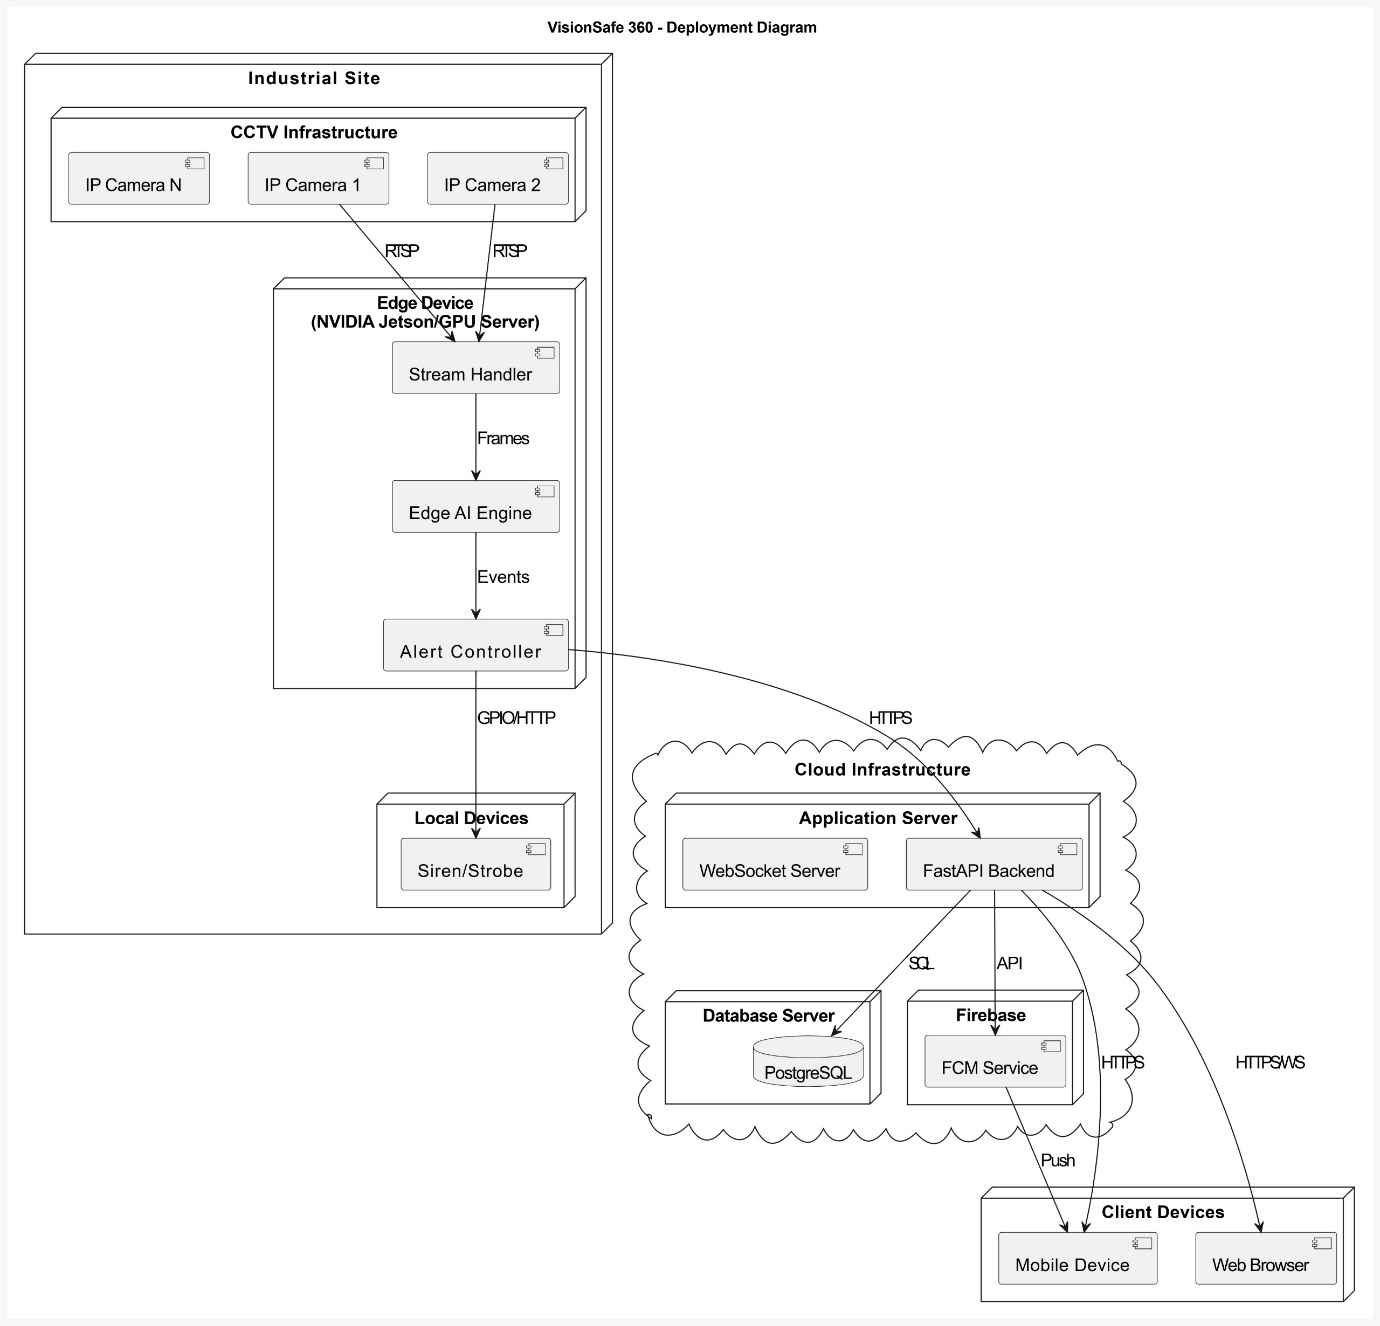
\includegraphics[width=0.95\linewidth,height=0.72\textheight,keepaspectratio]{images/img_016.jpeg}
\caption{Deployment Diagram}
\end{figure}

\section{API Specification Summary}

The communication between the Edge module, Dashboard, and Mobile App is mediated by a RESTful API. The following summary outlines the primary endpoints, all secured via JWT authentication:

POST /auth/login: Authenticates users and returns access tokens.

GET /cameras/health: Returns real-time status (Online/Offline/FPS) of all streams.

POST /incidents: Internal endpoint for the Edge Engine to upload new emergency incidents (generally high-severity PPE, fall, and proximity hazards).

PATCH /incidents/\{id\}: Used by Supervisors to update incident status and add "Action Taken" notes.

WS /events: A WebSocket endpoint providing a live feed of emergency incident events to the dashboard.

(Optionally) POST /ergonomics: Internal endpoint for uploading \textbf{non-emergency, low-severity posture records and ergonomic risk scores} for trend analysis, feeding dashboards and reports rather than immediate emergency alerting.

\section{Chapter Summary}

This chapter provided a comprehensive analysis of VisionSafe 360. It defined the problem scope, analyzed operational constraints, and detailed the functional and non-functional requirements necessary for a robust safety solution. The system architecture-prioritizing \textbf{Edge computing} for latency and privacy—was modeled through standard UML diagrams (Use Case, Activity, Class, Sequence) and Data Flow Diagrams.

The design incorporates a \textbf{unified, AI-driven hazard detection pipeline} covering four hazard categories: \textbf{PPE detection}, \textbf{fall detection}, \textbf{unsafe proximity monitoring}, and \textbf{Posture-related Ergonomic Risk Analysis}. A severity-aware alerting policy clearly distinguishes between emergency incident handling—reserved for high-severity, acute hazards—and continuous, preventive ergonomic risk monitoring for posture-related hazards. Within this architecture, acute hazards (PPE violations, falls, unsafe proximity) drive the real-time emergency alerting workflow, whereas posture-related ergonomic deviations are continuously monitored and recorded as low-severity events for long-term trend analysis and preventive ergonomics, thereby supporting HSE teams without introducing additional alert fatigue. These design specifications lay the groundwork for \textbf{Chapter 4}, which will detail the implementation of the inference pipelines, backend services, and interface integration.
